\chapter{ペンローズ図と現実のブラックホールの形成}

クラスカル図はシュヴァルツシルト地平線の近傍を巧みに記述するが、現実のブラックホールは永遠に存在するわけではない。物質が崩壊するときに形成されるのである。拡張された図のどの部分が、その物理的な歴史を経てもなお生き残るのだろうか。この問いに答えるには、時空全体を収めるのに十分大きく、かつ光の運動を保つのに十分に統制された図が必要である。まず平坦な時空をコンパクト化し、次にシュヴァルツシルト時空をコンパクト化し、最後に落下する放射の殻を挟んで適切な部分同士を縫い合わせる。

\section{地平線近傍：クラスカルの復習と四つの領域}

前回の講義が終わったまさにその地点から始める。シュヴァルツシルト地平線のごく近くでは、幾何学は局所的に平坦空間のように見える。地平線自体は、通常のミンコフスキー時空中で加速座標がそうであるように、双曲的な極座標の軌跡のように振る舞う。この局所的な描像において、我々は最初から一つの規則を課し、決して緩めない。すなわち、動径方向の光線は\(45^\circ\)で描かれ、あらゆる時間的worldlineはそれらのヌル線より急でなければならない。

この復習で用いる座標は、落下する観測者から見た時間と空間と考えるのが最もよい。それらの局所慣性座標では、地平線の近傍はほとんど平坦に見える。しかし、穴の外側で固定された半径にとどまることに固執する観測者は慣性系にいない。落下する系に対して、そのような人物は加速された曲線を描く。地平線に近いところでとどまるほど、外にとどまるために必要な加速度は大きくなる。これが、板の右側に描かれた外部曲線の族の物理的内容である。

\begin{figure}[htbp]
\centering
\includegraphics[width=0.72\textwidth]{lecture_08_figure_02.png}
\caption{地平線近傍の四領域幾何学の板書スケッチ。外部の赤い曲線は、固定された半径におけるホバリングするworldlineの族を記録している。}
\lectureframe{00:02:54}
\end{figure}

\begin{figure}[htbp]
\centering
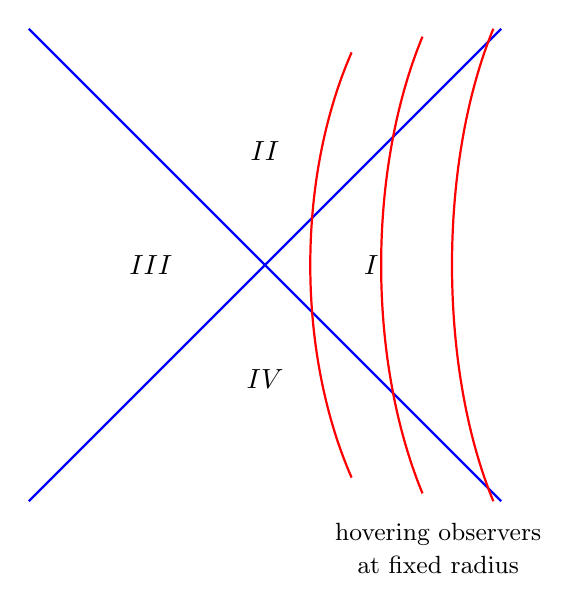
\begin{tikzpicture}[scale=1.0]
\draw[thick,blue] (-3,3) -- (3,-3);
\draw[thick,blue] (-3,-3) -- (3,3);

\draw[red,thick] (1.1,-2.7) .. controls (0.4,-1.1) and (0.4,1.1) .. (1.1,2.7);
\draw[red,thick] (2.0,-2.9) .. controls (1.3,-1.2) and (1.3,1.2) .. (2.0,2.9);
\draw[red,thick] (2.9,-3.0) .. controls (2.2,-1.3) and (2.2,1.3) .. (2.9,3.0);

\node at (1.35,0.0) {$I$};
\node at (0.0,1.45) {$II$};
\node at (-1.45,0.0) {$III$};
\node at (0.0,-1.45) {$IV$};

\node[align=center] at (2.2,-3.6) {\small hovering observers\\\small at fixed radius};
\end{tikzpicture}
\caption{復習で用いたクラスカル型の因果構造の清書。領域\(I\)は外部、領域\(II\)は脱出不可能な内部であり、領域\(III\)と\(IV\)は、後に現実の崩壊するブラックホールに対して破棄される形式的拡張に属する。}
\end{figure}

これだけでブラックホールが何をするか述べるのに十分である。外部領域\(I\)では、物体や信号は内向きに進むこともできるが、外側にとどまることも、外へ向きを変えることもできる。対照的に、領域\(II\)では因果的な判定は固定されている。ひとたび内部に入れば、外部へ戻る未来向きの因果的経路は存在しない。領域\(II\)からどちらかの外部領域へ脱出するには、どこかで\(45^\circ\)より浅い軌道が必要となり、したがって光より速くなければならない。許される未来向きの時間的軌道はすべて特異点で終わる。

この冒頭の復習は単なる繰り返しではない。本章の主要なテーマを準備するものである。クラスカル図は有用だが、そのすべてが現実のブラックホールに対して物理的に意味を持つわけではない。

\begin{classroomqa}
\audiencequestion{この図の軸は何であり、赤い曲線は誰の固定位置worldlineなのか。}
\lecturerresponse{軸は、自由落下する観測者にとって自然な座標における時間と空間である。地平線の近くでは、その観測者はほとんど通常の平坦な時空を見る。一方、赤い定位置曲線は、穴の外側で静止させられた観測者のものである。それらは加速されたworldlineであり、必要な加速度は地平線に近づくほど大きくなる。
\lecturetimestamp{00:05:58--00:06:47}}
\end{classroomqa}

\section{なぜコンパクト化するのか：無限の時空から有限の黒板へ}

次の手順は方法論的なものである。これらの図におけるヌル方向は無限遠へ延び、時間自体も同様である。したがって、座標を変えない限り、時空全体を通常の黒板に描くことはできない。講師の動機はきわめて具体的である。すべてを一度に見て大域的な因果構造について推論したいなら、光線を認識可能に保ちながら無限の時空を有限の領域に圧縮する方法が必要である。

そこで彼は易しい場合、すなわちおなじみの平坦な時空に立ち返る。関心のある問題は球対称であるから、角度方向を抑え、時間と動径座標のみを保つ。座標\(T\)と\(R\)を用い、
\[
R\ge 0,
\]
とする。極座標において負の動径距離は意味を持たないからである。また単位を
\[
c=1.
\]
と選ぶ。この規約のもとで、動径方向のヌル運動は\(45^\circ\)で描かれる。

コンパクト化写像を導入する前に、講義はしばらく\(T\)-\(R\)平面の中で我々の向きを定める。時間軸、動径軸、いくつかの等時間スライス\(T=0,\pm1,\pm2\)、そしていくつかの等動径線\(R=1,2,3\)を描く。これは無意味な形式主義ではない。我々に目印を与え、後に図を有限の大きさに押し込むときに、どの特徴を保ちたいのかを明らかにするのである。

原点についても、微妙だが重要な教育的な点がある。簡約された動径描像では、ちょうど\(R=0\)を狙った光線は原点で跳ね返って戻ってくるように見える。しかし物理的に壁で反射しているわけではない。完全な球対称幾何では、光線は単に原点を通り抜けて反対側へ出ていく。見かけの跳ね返りは、半平面\(R\ge 0\)で扱っていることの帰結にすぎない。

同様に、原点を外した光線は、最初はほとんど同じに見え、最近接点に達し、それから外側へ向きを変える。この座標では、何かが原点からそれを斥けたかのようにさえ見えるかもしれない。しかしそれもまた、よく知られた角運動量障壁の座標による記述であって、新しい力ではない。講師はこれらの例に時間を割く。図を変形する前に、聴衆にその図を信頼してほしいからである。

ここで本質的な操作が来る。我々は図を押し縮め、引き伸ばすが、一つのことは固定しておく。動径光線は\(45^\circ\)線のままでなければならない。これがコンパクト化の要点のすべてである。

\begin{classroomqa}
\audiencequestion{選ばれた原点に物理的に特別なものはあるのか、また、見かけ上曲がった光線はそこに力がある証拠なのか。}
\lecturerresponse{いいえ。この段階では、原点は球座標によって選ばれた中心にすぎない。見かけの跳ね返りと曲がりは、完全な空間的運動を\(R\geq0\)に簡約したことから生じる。対称性は、太陽の場合のように、中心を便利にすることがあるが、座標の選択がそこにブラックホールや反射壁を置くわけではない。
\lecturetimestamp{00:16:27--00:17:08}}
\end{classroomqa}

\section{ヌル座標とペンローズ形式における平坦時空}

変形を精密にするために、ヌル座標を導入する。ここが講義の数学的に整った部分であり、板書はその操作を明示する。

\begin{figure}[htbp]
\centering
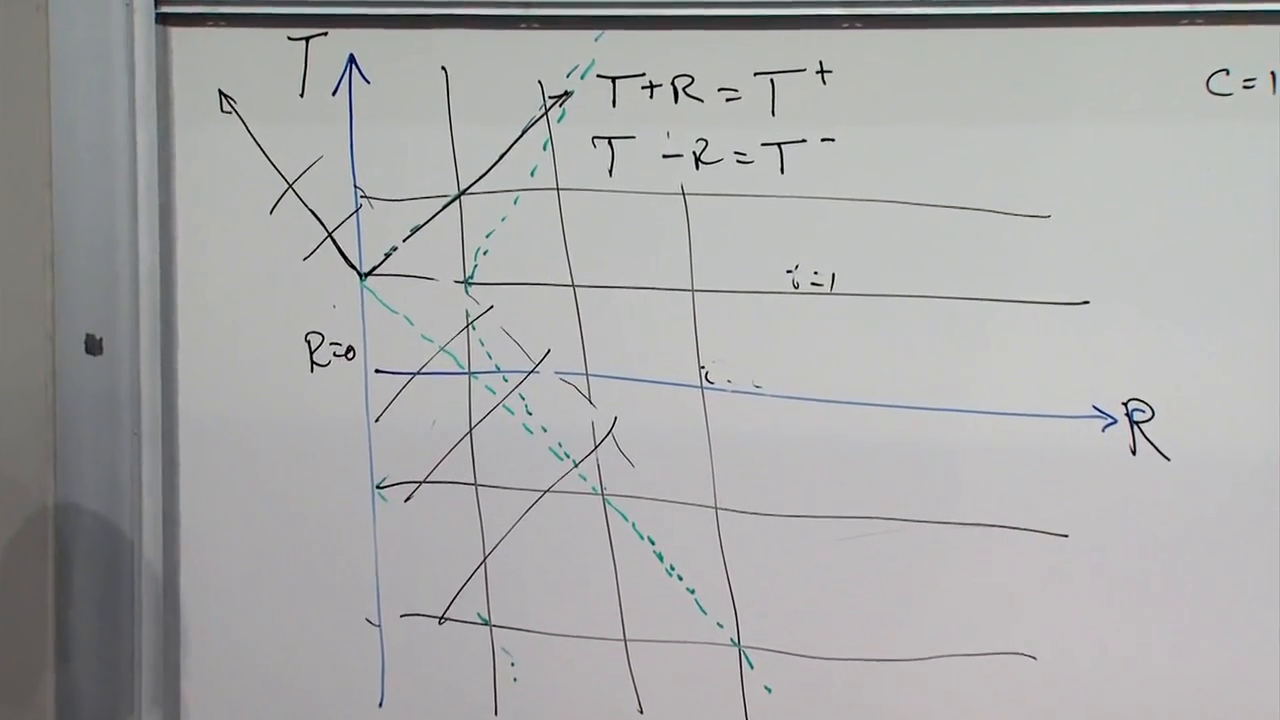
\includegraphics[width=0.82\textwidth]{lecture_08_figure_03.png}
\caption{\(T^+=T+R\)と\(T^-=T-R\)の導入時の、遮るもののない\(T\)-\(R\)ボード。簡約された動径原点は青い縦線\(R=0\)である。}
\lectureframe{00:19:45}
\end{figure}

我々は
\begin{align}
T^+ &= T+R, \\
T^- &= T-R.
\end{align}
と定義する。これらは動径ヌル運動に適合している。内向きの動径光線は\(T^+=\text{const}\)をもち、一方、外向きの動径光線は\(T^-=\text{const}\)をもつ。

\paragraph{導出の実演。}
直線\(R=0\)はこれらの座標で特に簡単になる。実際、
\begin{align}
R=0
&\iff T+R=T-R \\
&\iff T^+=T^-.
\end{align}
したがって、時間的境界\(R=0\)の全体は単一の関係
\begin{equation}
R=0 \iff T^+=T^-.
\end{equation}
によって記述される。

\begin{figure}[htbp]
\centering
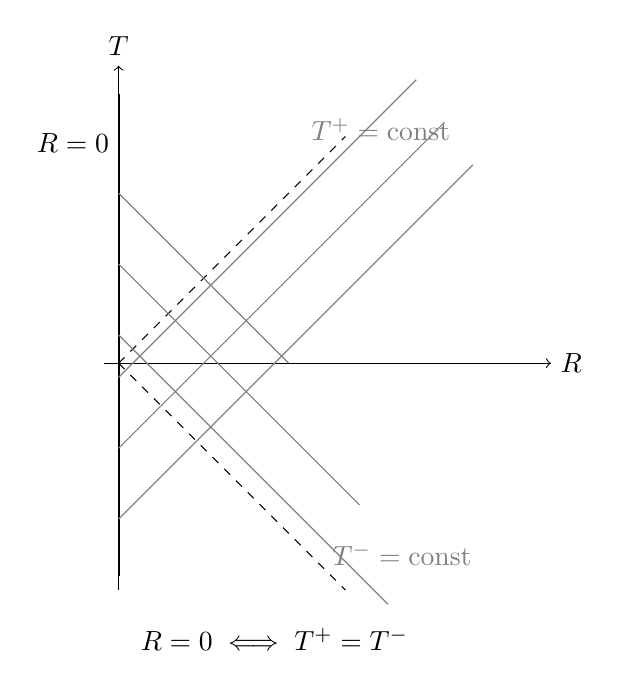
\begin{tikzpicture}[scale=0.9]
\draw[->] (-0.2,0) -- (6.1,0) node[right] {$R$};
\draw[->] (0,-3.2) -- (0,4.2) node[above] {$T$};

\draw[thick] (0,-3.0) -- (0,3.8);
\node[left] at (0,3.1) {$R=0$};

\draw[dashed] (0,0) -- (3.2,3.2);
\draw[dashed] (0,0) -- (3.2,-3.2);

\draw[gray] (0,2.4) -- (2.4,0);
\draw[gray] (0,1.4) -- (3.4,-2.0);
\draw[gray] (0,0.4) -- (3.8,-3.4);

\draw[gray] (0,-2.2) -- (5.0,2.8);
\draw[gray] (0,-1.2) -- (4.6,3.4);
\draw[gray] (0,-0.2) -- (4.2,4.0);

\node[gray] at (3.7,3.3) {$T^+=\mathrm{const}$};
\node[gray] at (4.0,-2.7) {$T^-=\mathrm{const}$};

\node at (2.2,-3.9) {$R=0 \iff T^+=T^-$};
\end{tikzpicture}
\caption{整った\(T\)-\(R\)の描き直し。二つのヌル族は\(T^+\)と\(T^-\)のレベル集合であり、直線\(R=0\)は同値に\(T^+=T^-\)である。}
\end{figure}

次にコンパクト化する。二つの新しいヌル座標\(U^\pm\)を導入し、それぞれを対応する\(T^\pm\)から同じ有界単調関数\(F\)によって得る：
\begin{align}
U^+ &= F(T^+), &
U^- &= F(T^-),
\end{align}
ここで
\begin{equation}
F(+\infty)=1,
\qquad
F(-\infty)=-1.
\end{equation}
講義で便利な選択は
\begin{equation}
F(x)=\tanh x,
\end{equation}
であり、したがって
\begin{equation}
U^+ = \tanh(T^+),
\qquad
U^- = \tanh(T^-).
\end{equation}
双曲線正接に神聖なものは何もない。それは正しい極限挙動をもつ滑らかな関数にすぎず、それによって無限の座標範囲を有限の範囲へ押し縮めるのである。

ヌル構造が保たれる理由は単純である。内向きの動径光線が\(T^+=\text{const}\)をもつなら、
\[
U^+=F(T^+)=\text{const},
\]
であり、同様に外向きの動径光線が\(T^-=\text{const}\)をもつなら、
\[
U^-=F(T^-)=\text{const}.
\]
である。したがってコンパクト化は二つのヌル方向を別々に再パラメータ化し、動径光線は\(45^\circ\)線のままである。原点線も同じようにきれいに運ばれる：
\[
T^+=T^- \Longrightarrow U^+=U^-.
\]

この時点で、平坦時空の無限半平面は有限の三角形に圧縮された。次に講義はその辺の読み方を教える。空間的無限遠は単一の点\(i^0\)に崩壊する。未来と過去の時間的無限遠は\(i^+\)と\(i^-\)である。二つのヌル辺は\(\mathcal{I}^+\)と\(\mathcal{I}^-\)であり、しばしばスクリプラス、スクリマイナスと発音され、入射光線と出射光線が始まり終わる場所である。

\begin{figure}[htbp]
\centering
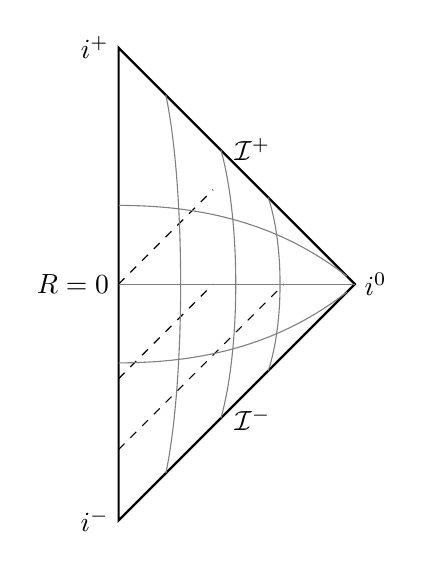
\begin{tikzpicture}[scale=1.0]
\draw[thick] (0,-3) -- (0,3) -- (3,0) -- cycle;

\node[left] at (0,3) {$i^+$};
\node[left] at (0,-3) {$i^-$};
\node[right] at (3,0) {$i^0$};
\node[left] at (0,0) {$R=0$};
\node[above right] at (1.35,1.45) {$\mathcal{I}^+$};
\node[below right] at (1.35,-1.45) {$\mathcal{I}^-$};

\draw[dashed] (0,-2.1) -- (2.1,0.0);
\draw[dashed] (0,-1.2) -- (1.2,0.0);
\draw[dashed] (0,0.0) -- (1.2,1.2);

\draw[gray] (0,0) -- (3,0);
\draw[gray] (0,1.0) .. controls (1.0,1.0) and (2.0,0.8) .. (2.9,0.1);
\draw[gray] (0,-1.0) .. controls (1.0,-1.0) and (2.0,-0.8) .. (2.9,-0.1);

\draw[gray] (0.6,-2.4) .. controls (0.85,-1.2) and (0.85,1.2) .. (0.6,2.4);
\draw[gray] (1.3,-1.7) .. controls (1.55,-0.8) and (1.55,0.8) .. (1.3,1.7);
\draw[gray] (1.9,-1.1) .. controls (2.1,-0.5) and (2.1,0.5) .. (1.9,1.1);
\end{tikzpicture}
\caption{動径的に簡約された平坦時空のペンローズ図。等時間曲線は\(i^0\)へ向かって外側へ走り、等動径曲線は\(i^-\)から\(i^+\)へ向かって立ち上がる。}
\end{figure}

講義からの最後の一点を心に留めておくべきである。これらの図は計量的大きさを\emph{保存しない}。それらは因果構造を保存する。それこそ我々が求めている不変量である。

\begin{classroomqa}
\audiencequestion{コンパクト化された等時間線は直線であるべきなのか。}
\lecturerresponse{選ばれた写像に対して直線となるのは対称なスライス\(T=0\)のみである。他の定\(T\)曲線は曲がり、その詳細な形状はコンパクト化関数に依存する。ごく遅い時刻のスライスは、通常の時間が際限なく続くにもかかわらず、上側の境界にますます近づいて密集する。
\lecturetimestamp{00:29:11--00:30:12}}
\end{classroomqa}

\section{コンパクト化されたシュヴァルツシルト幾何学}

平坦空間の構成を手に入れたので、ここでブラックホールに戻り、同じことをもう一度行う。ヌル座標を導入して無限の範囲を有限の図形に押し込むことにより、クルスカル幾何学をコンパクト化する。講師はその結果を、対角線状の長方形、すなわちダイヤモンドのような因果的描像と表現する。事象の地平面はヌル境界として現れ、外部に静止する世界線はその外側にとどまり、内部領域は今や紙面上で可視となった特異点で終端する。

決定的な物理的要点は、落下する観測者の経験において特異点が無限遠にあるのでは\emph{ない}ということである。事象の地平面を一度越えれば、特異点に衝突するまでの残りの固有時間は有限である。ペンローズ図はこのことを視覚的に避けがたく示している。

事象の地平面は再びシュヴァルツシルト条件
\begin{equation}
1-\frac{2MG}{r}=0
\qquad \Longleftrightarrow \qquad
r=2MG.
\end{equation}
によって同定される。等式\(r=2MG\)は、シュヴァルツシルト因子が符号を変える半径を印づける。

\begin{figure}[htbp]
\centering
\includegraphics[width=0.72\textwidth]{lecture_08_figure_04.png}
\caption{形式的な拡張描像と物理的に関連するブラックホール領域を対比する板書のスケッチ。赤いラベル\emph{特異点}が板上で明示されている。}
\lectureframe{00:37:59}
\end{figure}

\begin{figure}[htbp]
\centering
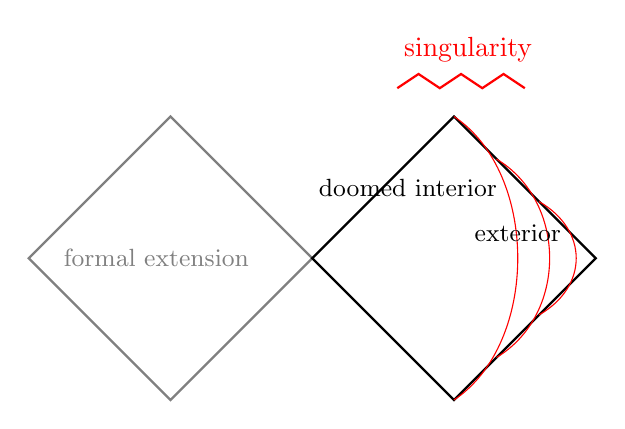
\begin{tikzpicture}[scale=0.9]
\draw[gray,thick] (-4,0) -- (-2,2) -- (0,0) -- (-2,-2) -- cycle;
\draw[thick] (0,0) -- (2,2) -- (4,0) -- (2,-2) -- cycle;

\draw[red,thick] (1.2,2.4) -- (1.5,2.6) -- (1.8,2.4) -- (2.1,2.6) -- (2.4,2.4) -- (2.7,2.6) -- (3.0,2.4);
\node[red] at (2.2,2.95) {singularity};

\draw[red] (2.0,-2.0) .. controls (3.2,-1.2) and (3.2,1.2) .. (2.0,2.0);
\draw[red] (2.6,-1.4) .. controls (3.6,-0.8) and (3.6,0.8) .. (2.6,1.4);
\draw[red] (3.2,-0.8) .. controls (3.9,-0.4) and (3.9,0.4) .. (3.2,0.8);

\node at (2.9,0.35) {\small exterior};
\node at (1.35,1.0) {\small doomed interior};
\node[gray] at (-2.2,0.0) {\small formal extension};
\end{tikzpicture}
\caption{講義で強調された因果的描像を慎重に描き直したもの。生き残る外部、運命づけられた内部、未来の特異点、そして拡張の余分な形式的部分との対比。}
\end{figure}

講義はここで非常に直接的である。あなたが外部にいるなら、依然として脱出できるかもしれないし、落ち込むかもしれない。あなたが内部にいるなら、あなたは運命づけられている。この図は、未来向きの因果的運動について重要なことすべてをすでに語っている。

象限\(III\)と\(IV\)は、最大に拡張されたクルスカル解の正統な部分である。領域\(III\)は第二の外部を与え、領域\(IV\)は時間反転されたブラックホール領域である。しかしながら、それらは崩壊によって作られた通常のブラックホールの時空には現れない。拡張解が数学的に教訓的なのは、まさに崩壊の構成がどの部分を捨て去らねばならないかを示してくれるからである。

\section{空間的スライス、二球面、そしてアインシュタイン--ローゼン橋}

ここでコンパクト化された図を空間的スライス上で凍結し、そのスライスが時空としてではなく\emph{空間}としてどのように見えるかを問う。ここでワームホールのイメージが入り込み、ここで空間的描像が因果的議論を追い越すことを許してはならない。

角度方向が抑圧されているので、動径図の各点は二球面を表す。シュヴァルツシルト半径\(r\)において、その面積は
\begin{equation}
A=4\pi r^2.
\end{equation}
である。したがって空間的スライスは、単なる一次元曲線ではなく、二球面の族である。その大きさはスライスに沿って移動するにつれて変化する。

遠方では球面は非常に大きい。内側へ移動するにつれて、その半径は収縮し、事象の地平面において最小値に達する。
\begin{equation}
r_{\min}=2MG.
\end{equation}
形式的な拡張を通り抜け続けるなら、球面は別の漸近的な側へ向かって再び膨張する。これがアインシュタイン--ローゼン橋の描像である。

\begin{figure}[htbp]
\centering
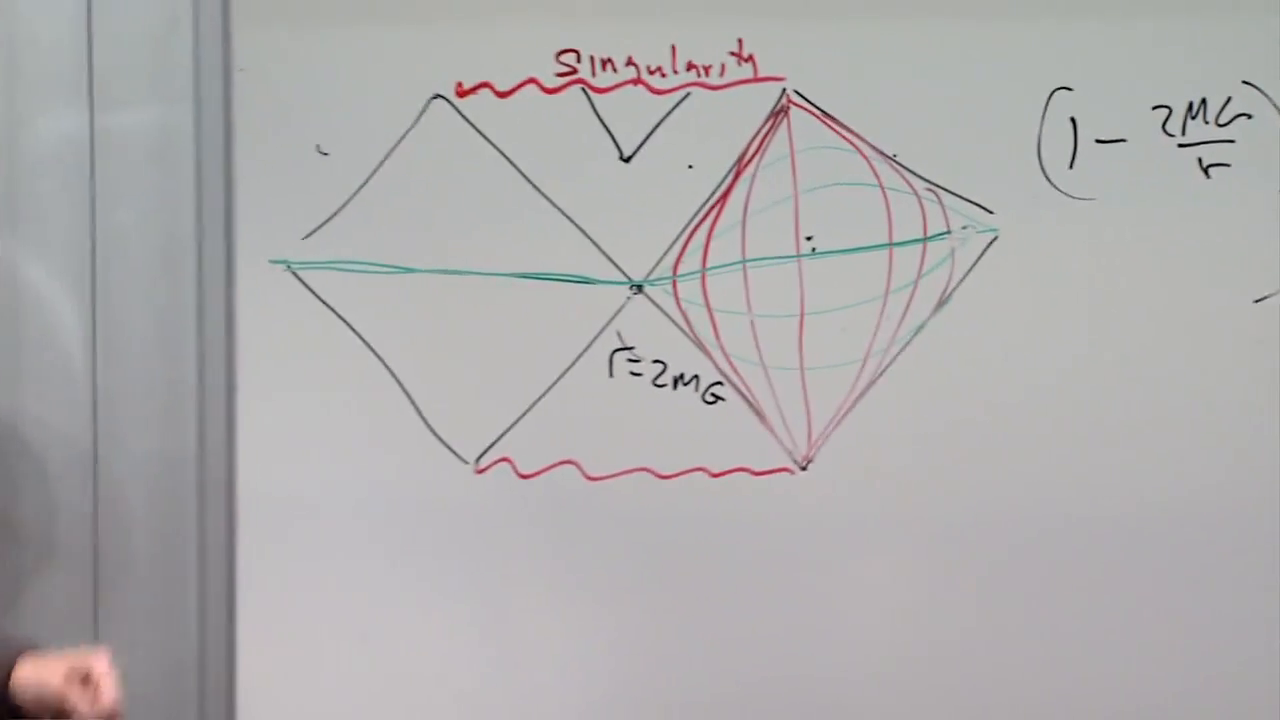
\includegraphics[width=0.72\textwidth]{lecture_08_figure_05.png}
\caption{橋の幾何学を構成するために用いられた緑の空間的スライスを伴う拡張クルスカル図。そのスライス上の各点は二球面を表し、その最小半径は\(r=2MG\)と印づけられている。}
\lectureframe{00:41:30}
\end{figure}

板書は関連するシュヴァルツシルト因子の一部のみを示しており、
\begin{equation}
1-\frac{2MG}{r},
\end{equation}
のどは同じ特別な半径\(r=2MG\)で生じる。

\begin{figure}[htbp]
\centering
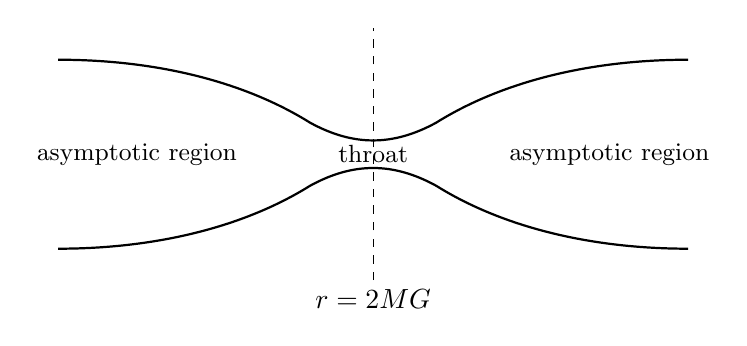
\begin{tikzpicture}[scale=1.0]
\draw[thick] (-4,1.2)
.. controls (-2.7,1.2) and (-1.6,0.9) .. (-0.8,0.4)
.. controls (-0.25,0.1) and (0.25,0.1) .. (0.8,0.4)
.. controls (1.6,0.9) and (2.7,1.2) .. (4,1.2);

\draw[thick] (-4,-1.2)
.. controls (-2.7,-1.2) and (-1.6,-0.9) .. (-0.8,-0.4)
.. controls (-0.25,-0.1) and (0.25,-0.1) .. (0.8,-0.4)
.. controls (1.6,-0.9) and (2.7,-1.2) .. (4,-1.2);

\draw[dashed] (0,-1.6) -- (0,1.6);
\node[below] at (0,-1.6) {$r=2MG$};
\node at (0,0) {\small throat};
\node at (-3.0,0) {\small asymptotic region};
\node at (3.0,0) {\small asymptotic region};
\end{tikzpicture}
\caption{拡張シュヴァルツシルト幾何学を通る空間的スライスの模式図。これは講義の橋の描像を慎重に再構成したものであり、文字通りの埋め込み計算ではない。}
\end{figure}

ここで訂正が来る。このスライスは二つの漸近領域の間の橋を示唆し、それゆえ首を通り抜けることによって一方の宇宙から他方へ旅行できるかもしれないという考えを誘う。講義はまずその示唆を現れさせ、次にそれを因果的に打ち消す。一方の外部領域から他方へ行くには、世界線はペンローズ図上のどこかで\(45^\circ\)ヌル線より浅くなければならない。それは禁じられている。したがってアインシュタイン--ローゼン橋は通過不可能である。

講師はまた、なぜ空間的な描像が誤解を招きうるのかを強調する。それは\emph{ある瞬間の空間}の描像である。しかし、通り抜けるのに十分な因果的時間がそもそも存在しない。大まかに言えば、橋は何かが渡れる前に開いて閉じてしまう。さらに良いのは、単にペンローズ図に戻って因果的な答えを読み取ることである。

\section{落下するヌル殻から現実のブラックホールを構成する}

ここで講義は問題を完全に切り替える。もはや永遠のブラックホールの性質を読み取っているのではない。現実のブラックホールを構成しているのである。

モデルは単純さのために選ばれている。内部構造が乱雑な崩壊する星ではなく、入射する放射の薄い球対称殻を想像する。それは光の殻であり、したがって光速で内向きに進む。十分に小さい半径では、その殻上のエネルギーが十分に密集してブラックホールが形成される。

第二の要素は、一般相対論的な形での球殻定理である。

\paragraph{注意。} この講義で用いられる球対称殻に対して、内部領域は平坦な時空であり、外部領域はシュヴァルツシルトである。これが講義で用いられる操作的な球殻定理、すなわちビルクホフ型の主張である。ここでは証明されない。

講師はこれを動機づけるために、まずニュートン的な球殻定理を想起する。球殻の内部には重力場がなく、球殻の外部では場は中心の点質量と同じである。次に、ここで必要な唯一の形で対応する相対論的版を述べる。内部は平坦であり、外部はシュヴァルツシルトである。殻は動いてもよく、規則は同じである。

これで崩壊時空を構成するのに十分である。殻自体はヌルであるから、\(45^\circ\)に描かれなければならない。そのヌル線の一方の側では幾何学は平坦である。もう一方の側ではシュヴァルツシルトである。この規則は次のように要約できる。
\begin{equation}
\begin{aligned}
\text{inside shell} &= \text{flat spacetime},\\
\text{outside shell} &= \text{Schwarzschild geometry}.
\end{aligned}
\end{equation}

すると貼り合わせの処方はほとんど気恥ずかしいほど単純になる。

\begin{enumerate}
\item 平坦なペンローズ図を描き、入射する殻の内部の領域だけを残す。
\item シュヴァルツシルトのペンローズ図を描き、同じ殻の外部の領域だけを残す。
\item 間違った部分を捨てる。
\item 生き残った二つの部分を殻の軌道に沿って縫い合わせる。
\end{enumerate}

講義はまさにこのように黒板で進む。一方の図の間違った半分を捨て、もう一方の間違った半分を捨て、正しい半分を殻に沿って貼り合わせる。

\begin{figure}[htbp]
\centering
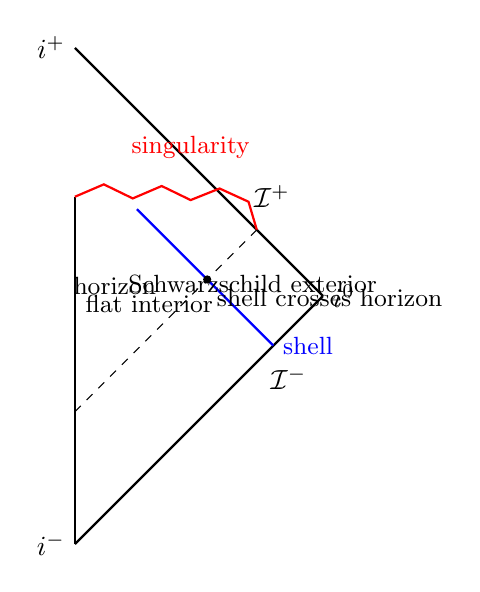
\begin{tikzpicture}[scale=1.05]
\coordinate (im) at (0,-3.0);
\coordinate (ip) at (0,3.0);
\coordinate (i0) at (3.0,0.0);
\coordinate (S)  at (0,1.2);
\coordinate (E)  at (2.2,0.8);
\coordinate (P)  at (2.4,-0.6);
\coordinate (Q)  at (0.75,1.05);
\coordinate (H)  at (0,-1.4);
\coordinate (X)  at (1.6,0.2);

\draw[thick] (im) -- (S);
\draw[thick] (im) -- (i0);
\draw[thick] (ip) -- (i0);

\draw[red,thick] (S) -- (0.35,1.35) -- (0.7,1.18) -- (1.05,1.33) -- (1.4,1.16) -- (1.75,1.30) -- (2.1,1.14) -- (E);
\node[red,above] at (1.4,1.55) {\small singularity};

\draw[thick,blue] (P) -- (Q);
\node[blue,right] at (P) {\small shell};

\draw[dashed] (H) -- (E);
\node[above left] at (1.1,-0.1) {\small horizon};

\filldraw (X) circle (1.2pt);
\node[below right] at (X) {\small shell crosses horizon};

\node at (0.9,-0.1) {\small flat interior};
\node at (2.15,0.15) {\small Schwarzschild exterior};

\node[left] at (im) {$i^-$};
\node[left] at (ip) {$i^+$};
\node[right] at (i0) {$i^0$};
\node[below right] at (2.25,-0.75) {$\mathcal{I}^-$};
\node[above right] at (2.05,0.95) {$\mathcal{I}^+$};
\end{tikzpicture}
\caption{崩壊幾何学の因果的再構成。殻は内向きのヌル線であり、平坦な時空はその内部側に、シュヴァルツシルト幾何学はその外部側に保たれる。}
\end{figure}

\begin{figure}[htbp]
\centering
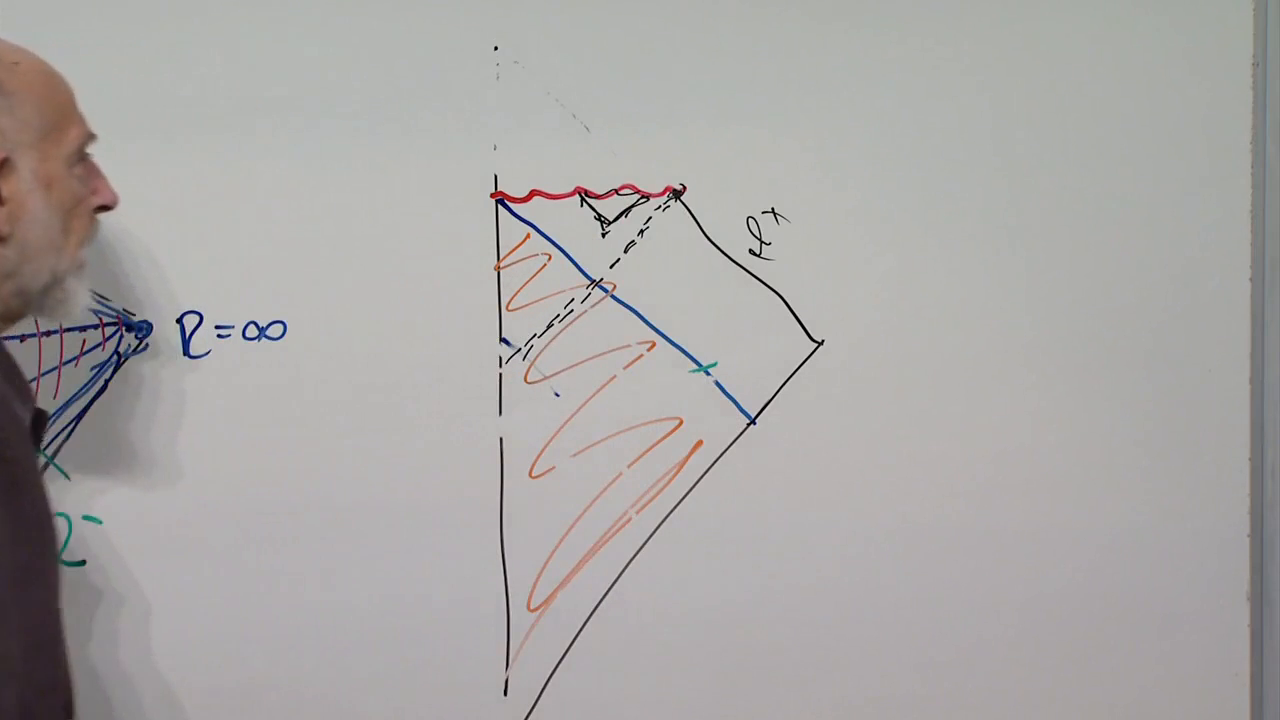
\includegraphics[width=0.76\textwidth]{lecture_08_figure_06.png}
\caption{平坦な内部とシュヴァルツシルト外部が青い落下する殻に沿って貼り合わされた後の、完成した黒板の構成。破線の\(45^\circ\)線は、特異点の未来の端点から逆向きにたどられ、事象の地平面を特定している。}
\lectureframe{00:57:30}
\end{figure}

殻自体は、単に図の平坦な部分からシュヴァルツシルトの部分へ横切っている瞬間に、何も特別なことを経験しない。それは光的な殻であり、特異点に達するまで内向きに進み続ける。本質的な構造は殻上の局所的な劇によってもたらされるのではなく、貼り合わされた時空の因果的組織によってもたらされる。

\begin{classroomqa}
\audiencequestion{崩壊する殻が自身のシュヴァルツシルト半径を横切るとき、不連続性はあるか。}
\lecturerresponse{いいえ。その横断で局所的に特異なことは何も起こらない。殻はそのヌル軌道を進み続ける。特別な出来事は因果的である。殻が自身の\(2MG\)半径を横切った後、未来向きの経路はもはやそれを無限遠に戻すことはできない。
\lecturetimestamp{00:56:19--00:56:42}}
\end{classroomqa}

\section{到着前の地平面：事象の地平面のパズル}

ここで講義の概念的頂点が来る。崩壊時空が構成されたなら、自然な問いはこうである。地平面はどこにあるのか。あるいは講師の言い方では、戻れない点はどこにあるのか。

\paragraph{定義。} 事象の地平面とは、\(\mathcal{I}^+\)へ未来向きの因果的信号を依然として送ることのできる事象と、そうでない事象との境界である。

講義はそれを図式的に見つける。特異点が未来のヌル無限遠と出会う角から始め、\(45^\circ\)のヌル線を逆向きにたどる。その逆向きにたどられたヌル線が事象の地平面である。

しかし講師はさらに第二の点を主張する。そしてそれが学生たちを不安にさせる点である。地平線は、殻が自身のシュヴァルツシルト半径を横切る瞬間に単に現れて、その後そのまま留まるのではない。拡大された板書の図では、地平線は中心付近の小さなトラップされた領域として始まり、まだ平坦な時空の一部を通って外側へ膨張し、その後になって初めて入射する殻と出会う。その出会いの事象において、殻は自身のシュヴァルツシルト半径を通過する。その事象より上では、地平線は完成したブラックホールの通常の一定半径の地平線である。

\begin{figure}[htbp]
\centering
\resizebox{0.96\linewidth}{!}{%
\begin{tikzpicture}[scale=1.08,>=Latex]
\coordinate (im) at (0,-3.0);
\coordinate (ip) at (0,3.0);
\coordinate (i0) at (3.0,0.0);
\coordinate (S)  at (0,1.2);
\coordinate (E)  at (2.2,0.8);
\coordinate (P)  at (2.4,-0.6);
\coordinate (Q)  at (0.75,1.05);
\coordinate (H)  at (0,-1.4);
\coordinate (X)  at (1.6,0.2);

\draw[thick] (im) -- (S);
\draw[thick] (im) -- (i0);
\draw[thick] (ip) -- (i0);

\draw[red,thick] (S) -- (0.35,1.35) -- (0.7,1.18) -- (1.05,1.33) -- (1.4,1.16) -- (1.75,1.30) -- (2.1,1.14) -- (E);
\node[red,above left] at (S) {\small singularity};

\draw[very thick,red] (H) -- (E);

\draw[thick,blue] (P) -- (Q);

\filldraw (X) circle (1.2pt);

\draw[gray] (0.0,-2.1) .. controls (0.85,-1.95) and (1.9,-1.3) .. (2.8,-0.2);
\draw[gray] (0.0,-1.2) .. controls (0.95,-1.0) and (1.8,-0.45) .. (2.45,0.35);
\draw[gray] (0.0,-0.2) .. controls (0.8,-0.05) and (1.45,0.35) .. (1.95,0.95);

\node[below right] at (2.28,-0.72) {$\mathcal{I}^-$};
\node[above right] at (2.12,0.92) {$\mathcal{I}^+$};

\draw[very thick,red] (3.2,-1.15) -- (3.75,-1.15);
\node[anchor=west] at (3.85,-1.15) {\small event horizon};
\draw[thick,blue] (3.2,-1.55) -- (3.75,-1.55);
\node[anchor=west] at (3.85,-1.55) {\small infalling shell};
\filldraw (3.48,-1.95) circle (1.2pt);
\node[anchor=west] at (3.85,-1.95)
  {\small shell reaches \(r=2MG\)};
\end{tikzpicture}
}
\caption{逆向きにたどった事象の地平線を強調した崩壊図。地平線の一部は、まだ局所的に平坦で殻がまだ到達していない領域にある。}
\end{figure}

これが、講義の残りが詳しく論じる際立った効果である。地平線の一部は平坦な時空にある。殻はまだそこに到着しておらず、観測者の過去光円錐上にも見えない。観測者は重力場を感じないが、それでも脱出できない。その理由は局所的な力ではない。それはその事象の大域的な因果的未来である。

\begin{classroomqa}
\audiencequestion{この構成は、殻を横切ることができないと言っているのか、それとも地平線を横切ることができないと言っているのか。地平線がまだその内側にあるとき、殻はどこにあるのか。}
\lecturerresponse{殻を横切ることはできる。地平線は別のヌル面である。すなわち、\(\mathcal I^+\)と通信できる事象とできない事象との境界である。入射する殻は、その全エネルギーに対応するシュヴァルツシルト半径を横切るときに、まさにその境界と出会う。出会いの前には、事象の地平線の一部は平坦な内部を通っている。出会いの後には、殻は完成したブラックホールの内側にある。
\lecturetimestamp{00:58:42--01:01:06}}
\end{classroomqa}

\begin{classroomqa}
\audiencequestion{内部が平坦で殻がまだ遠くにあるなら、なぜ地平線のすぐ内側にいる者は、殻が到着する前に地平線を横切って歩いていけないのか。}
\lecturerresponse{可能な限り最速の外向き世界線、すなわち\(45^\circ\)光線を描く。逆向きにたどった地平線の内側の事象からは、その光線でさえ入射する殻と出会うのが遅すぎて特異点で終わる。歩くのはさらに遅い。\emph{殻はまだ横切っていない}という表現は、時間座標が選ばれるまでは不完全である。因果図が座標に依存しない答えを与える。入射する宇宙マイクロ波背景放射は同じ例ではない。なぜならそれはこの幾何学を作り出す崩壊する球殻ではないからである。
\lecturetimestamp{01:01:07--01:04:03}}
\end{classroomqa}

\section{鏡と未来を変える試み}

ここで問いは図を実験室に変える。入射する光の殻がトラップされる前に反射できたとしよう。すると仮定された崩壊の履歴が変わり、事象の地平線も変わる。これは矛盾ではない。事象の地平線は、完全な時空の履歴が指定された後にのみ定義されるからである。

\begin{classroomqa}
\audiencequestion{もし完全に反射する鏡が、シュヴァルツシルト半径になるはずのすぐ外側に置かれ、殻が跳ね返って外へ出るとしたらどうか。}
\lecturerresponse{その理想化された履歴では、入射するヌル線は鏡で外向きに転じ、未来の境界に達する。元の図のブラックホールは形成されない。真に無重量の鏡は不可能であり、物理的な鏡はそれ自身の応力エネルギーに寄与するが、この思考実験は論理的な要点を示している。すなわち、殻が実際の事象の地平線を横切った後にのみ、脱出はもはや不可能になるのである。
\lecturetimestamp{01:04:33--01:05:54}}
\end{classroomqa}

\begin{classroomqa}
\audiencequestion{殻が来ることを知っている観測者が、急いで鏡や信号を送って殻を引き返させることができるだろうか。}
\lecturerresponse{必要な装置を十分早く地平線の外側に置ける場合に限る。アリスは、ボブが殻を送るよう事前に手配でき、したがって見る前に何が来るかを知ることができる。しかし、彼女の事象が地平線の内側に入ってしまえば、鏡も指示も必要な外部の点に間に合って到達できない。未来の実験についての知識は、図が禁じている因果経路を開かない。
\lecturetimestamp{01:05:55--01:08:18}}
\end{classroomqa}

\begin{classroomqa}
\audiencequestion{すでに事象の地平面の内側にある鏡はどうなるのか、また特異点はその未来において無限に遠いのか。}
\lecturerresponse{その鏡は、単に別の運命づけられた物体にすぎない。鏡は光を局所的に反射しうるが、反射された光も、鏡も、アリスも、すべて特異点で終わる。一般的な落下世界線は有限の固有時間でそこに到達する。無限に遠いのは、コンパクト化された図の理想的な上端の角だけである。その角の近くにとどまろうとすれば、無限の加速度とエネルギーが必要になる。さらに、固定された事象間では、加速された時計は慣性の時計よりも多くの固有時間を蓄積するのではなく、少ない固有時間しか蓄積しない。
\lecturetimestamp{01:08:19--01:10:19}}
\end{classroomqa}

\begin{classroomqa}
\audiencequestion{崩壊する殻が巨大であれば、殻の内側にいながら最終的な中心から遠く離れた人物は、殻が通過する間その場にとどまることができるのか。}
\lecturerresponse{はい、その人物の事象が依然として事象の地平面の外側にあるならば可能である。物質の殻の内側にいることは、ブラックホールの内側にいることと同じではない。放射は観測者に当たり、傷つけるかもしれないが、それは殻との局所的な相互作用であり、脱出という因果的な問題とは別である。
\lecturetimestamp{01:10:21--01:11:24}}
\end{classroomqa}

\section{時間スライスと成長する地平面}

曲がった時空における\emph{時間の瞬間}とは、選ばれた空間的超曲面を意味する。そのような曲面を積み重ねたものが葉層であり、各曲面に数を割り当てることで時間座標が定義される。異なる葉層は同じ崩壊図を異なる仕方で切る。それらはどの遠方の事象が同時であるかについては一致しないが、どのヌル光線が無限遠に到達するかは変えない。

\begin{figure}[htbp]
\centering
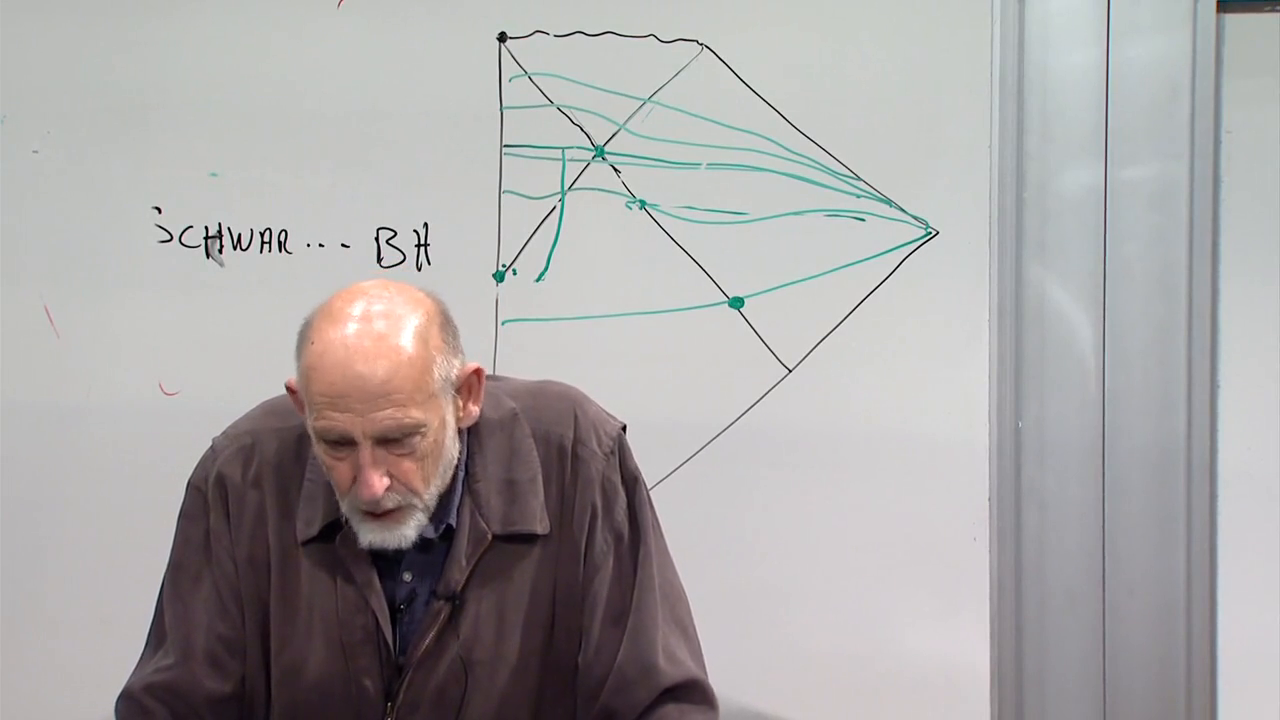
\includegraphics[width=0.77\textwidth]{lecture_08_figure_07.png}
\caption{複数の緑の空間的スライスを伴う後半の板書図。スライスは時間座標を与えるが、黒いヌル境界とそれらの因果関係はその選択に依存しない。}
\lectureframe{01:17:30}
\end{figure}

\begin{classroomqa}
\audiencequestion{ある一瞬において、観測者から地平面までの距離と、地平面から殻までの距離を比較することで、このパズルを言い換えることができるか。}
\lecturerresponse{葉層を選んだ後なら有用な直観になりうるが、\emph{ある一瞬において}という表現は座標に依存する。明確な構成は、空間的スライスの族を描くことである。初期のスライスは大きな殻と出会い、閉じ込められた中心領域はない。後期のスライスは、依然として落下中の殻の内側で成長する地平面と出会う。一つの特別なスライスは、殻が自身のシュヴァルツシルト半径を横切る事象を通る。
\lecturetimestamp{01:11:26--01:14:21}}
\end{classroomqa}

\begin{classroomqa}
\audiencequestion{地平面が外側へ開くにつれてシュヴァルツシルト半径は成長するのか、また殻がそれを横切った後もなぜ地平面は成長し続けるのか。}
\lecturerresponse{最終的なシュヴァルツシルト半径\(2MG\)は、全質量\(M\)が固定されているため固定されている。初期の空間的スライス上で成長するのは、地平面の断面の面積半径である。それは中心から始まり、\(r=2MG\)で殻と出会うまで増大し、その後停止する。出会いの事象より上では、地平面は一定の\(r\)の線\(r=2MG\)である。ただしコンパクト化によってその線が垂直に見えたり、計量的に一様に見えたりするわけではない。
\lecturetimestamp{01:14:22--01:16:15}}
\end{classroomqa}

\begin{classroomqa}
\audiencequestion{最終的なシュヴァルツシルト半径の半分の位置に最初にいる観測者はどうなるのか。その観測者は殻が到着したときにのみ重力を感じるべきではないのか。}
\lecturerresponse{そのとおりである。その観測者は、依然として平坦な時空にいるうちに、成長する事象の地平面を最初に横切るが、突然の力を感じることはない。落下する放射殻は物質であり、後に感じられるかもしれないが、事象の地平面はそうではない。それを横切るということは、未来向きの因果的経路がすべて今や無限遠に到達しないということを意味するにすぎない。まさにその意味で、地平面は幽霊のようなものである。
\lecturetimestamp{01:16:17--01:17:45}}
\end{classroomqa}

\begin{classroomqa}
\audiencequestion{十分早く出発した観測者は、成長する地平面よりも速く外側へ移動して脱出できるか。}
\lecturerresponse{はい。地平面の外側の事象には\(\mathcal I^+\)への外向きの因果的経路が存在するが、内側の事象には存在しない。選んだスライス上では、利用可能な動径距離と、到来する殻が経路を閉ざすまでの時間を比較できるが、厳密な判定を与えるのはヌル線である。物質的な地平面が外側へ突進してくるのを観測者が見ることはない。なぜなら、見るべき局所的な表面が存在しないからである。
\lecturetimestamp{01:17:46--01:18:54}}
\end{classroomqa}

\section{図が保存するもの}

ページ上の形は、縮尺図として読んではならない。小さな角が時空の無限の領域を表すこともあり、大きな区画が控えめな物理的間隔を表すこともある。コンパクト化は、ヌル方向を保存するために、計量的な大きさを意図的に犠牲にする。生き残るのは因果関係である。すなわち、誰が誰に信号を送れるか、どの事象がどの他の事象に影響を与えうるか、そしてどの世界線が光速の限界によって閉じ込められるかである。

\begin{classroomqa}
\audiencequestion{この図が長さと時間をそれほどひどく歪めるなら、それは何を忠実に表しているのか。}
\lecturerresponse{それは光線、したがって因果構造を表している。事象の地平面を特定するには、最後の外向きヌル光線を未来の無限遠から逆向きにたどればよい。ページ上の見かけの距離から答えを推測しようとするのは信頼できない。いったん因果図が描かれれば、信号、脱出、戻れないことに関する問いには、計量のスケールが抑圧されていても幾何学的な答えがある。
\lecturetimestamp{01:18:56--01:21:45}}
\end{classroomqa}

\begin{classroomqa}
\audiencequestion{ペンローズ図を直観的に使えるようになるには、どれくらい慣れる必要があるのか。}
\lecturerresponse{長くはかからない。実践的な処方は、それらを描き、ヌル線をたどり、可能な世界線を試して、因果的な制約に慣れるまで確かめることである。ここでの直観は、図を使わずに推測するのではなく、図を扱うことによって獲得される。
\lecturetimestamp{01:21:49--01:22:05}}
\end{classroomqa}

\begin{classroomqa}
\audiencequestion{この視覚的な方法は、数学がしばしば図よりも信頼できる量子力学とは正反対なのか。}
\lecturerresponse{かなりの程度、そのとおりである。一般相対性理論は古典物理学である。四次元の曲がった時空を文字どおり描くのは難しく、ペンローズ図も依然として抽象的だが、その因果幾何学は、量子力学の根底にある実在よりもはるかに遠くまで描き、探求することができる。その違いが、これらの図をこれほど強力にしている理由の一部である。
\lecturetimestamp{01:22:05--01:22:58}}
\end{classroomqa}